\section{Modelo Supervisado}

Se modeló un algoritmo de aprendizaje automático capaz de aprender los patrones históricos de la cartera y predecir la probabilidad de que una nueva cohorte transite hacia el deterioro. El problema se define matemáticamente como una tarea de clasificación multiclase, donde se busca estimar la probabilidad condicional $P(Y=k \mid X=x^{(i)})$, siendo $X$ el vector de características de 10 dimensiones reducido en el capítulo anterior, y $Y \in \{1, 2, 3\}$ el espacio correspondiente a las etapas de riesgo definidas por la NIFBdM C-16.

\subsection{Estrategia de Evaluación y Desbalance de Clases}
El análisis exploratorio confirmó un desbalance de clases severo: la Etapa 1 (riesgo bajo) agrupa aproximadamente el 81\% de la muestra. Bajo esta asimetría, utilizar la Exactitud (\textit{Accuracy}) como métrica de éxito resulta engañoso; un clasificador trivial alcanzaría un 81\% de exactitud simplemente asignando a todas las cohortes la categoría de riesgo bajo.

Para las instituciones financieras, el costo de un Falso Negativo (clasificar una cartera altamente riesgosa como una de riesgo bajo) es por mucho, superior al de un Falso Positivo (sobreestimar el riesgo de una cohorte). Por consiguiente, la evaluación del modelo priorizarán la métrica de \textbf{Sensibilidad (\textit{Recall})} para las Etapas 2 y 3, garantizando la detección temprana del deterioro estructural, aun si esto implica un decremento en la Precisión (\textit{Precision}). Adicionalmente, se utilizará el Área Bajo la Curva ROC (AUC) para medir la capacidad de separación matemática entre clases.

\subsection{Preprocesamiento y Partición de Datos}
Se aplicó un muestreo aleatorio estratificado, dividiendo los datos en tres subconjuntos: Entrenamiento (64\%), Validación (16\%) y Prueba (20\%). 

Posteriormente, se aplicaron transformaciones matemáticas calibradas exclusivamente sobre el conjunto de entrenamiento:
\begin{itemize}
	\item \textbf{Variables Continuas:} Se utilizó un escalamiento (\textit{RobustScaler}), el cual sustrae la mediana y divide por el rango intercuartílico, protegiendo los gradientes contra la extrema asimetría de las magnitudes monetarias.
	\item \textbf{Variables Categóricas:} Se le aplicó codificación \textit{One-Hot}, expandiendo la dimensionalidad de entrada a un vector final de 71 dimensiones ($d=71$).
\end{itemize}

Para abordar el desbalance, se calculó un vector de pesos inversamente proporcional a las frecuencias de clase. Este vector penaliza los errores matemáticos cometidos sobre la clase minoritaria. Matemáticamente, el modelo penaliza aproximadamente 10 veces más un error de clasificación en la Etapa 3 que en la Etapa 1 (esto para evitar al máximo, los Falsos Positivos).

\subsection{Línea Base: Regresión Logística Multiclase}
Para establecer un umbral de desempeño, se entrenó un modelo estadístico lineal de Regresión Logística. Los resultados reflejaron las limitaciones de los modelos lineales ante dinámicas financieras complejas. A pesar de incorporar los pesos compensatorios, el modelo apenas logró un \textit{Recall} del 42\% para la Etapa 3. Las fronteras del riesgo demostraron no ser linealmente separables, haciendo necesario la transición hacia modelos no lineales.

\subsection{Arquitectura de la Red Neuronal Multicapa (MLP)}
Se seleccionó el \textit{framework} PyTorch para implementar una Red Neuronal Profunda, dada su escalabilidad y la flexibilidad para manipular directamente la función de pérdida. La arquitectura diseñada consta de:
\begin{enumerate}
	\item \textbf{Capa de Entrada:} El vector multidimensional ($X \in \mathbb{R}^{71}$).
	\item \textbf{Capas Ocultas:} Dos capas secuenciales (128 y 64 neuronas) con funciones de activación no lineales ReLU (\textit{Rectified Linear Unit}).
	\item \textbf{Regularización:} Para evitar el sobreajuste (\textit{overfitting}), se intercalaron capas de \textit{Dropout} con una probabilidad de apagado neuronal del 30\%.
	\item \textbf{Capa de Salida y Optimización:} Un vector de tres dimensiones que representa cada etapa de riesgo.
\end{enumerate}
Además, para cuantificar el error en cada etapa, para la función de pérdida usamos Entropía Cruzada Categórica, la cuál internaliza los pesos de desbalance, y como optimizador el algoritmo Adam.

El ciclo de aprendizaje se ejecutó mediante descenso de gradiente por mini-lotes (\textit{Mini-Batch Gradient Descent}). El monitoreo de la pérdida, demostró la ausencia de sobreajuste: la pérdida del conjunto de validación descendió simétricamente a la pérdida de entrenamiento durante 30 épocas, logrando una convergencia altamente estable.

\begin{table}[H]
	\centering
	\begin{tabular}{rcc}
		\hline
		\textbf{Época} & \textbf{Train Loss} & \textbf{Validation Loss} \\
		\hline
		01/30 & 0.9798 & 0.9512 \\
		02/30 & 0.9508 & 0.9383 \\
		03/30 & 0.9421 & 0.9313 \\
		04/30 & 0.9356 & 0.9259 \\
		05/30 & 0.9313 & 0.9247 \\
		\vdots & \vdots & \vdots \\
		25/30 & 0.9098 & 0.9060 \\
		26/30 & 0.9088 & 0.9064 \\
		27/30 & 0.9088 & 0.9058 \\
		28/30 & 0.9082 & 0.9043 \\
		29/30 & 0.9082 & 0.9056 \\
		30/30 & 0.9078 & 0.9053 \\
		\hline
	\end{tabular}
\end{table}

\subsection{Evaluación Final e Interpretación}
La red neuronal fue evaluada de manera definitiva sobre los 200,000 registros del conjunto de prueba, revelando una capacidad de generalización notablemente superior a la \textit{linebase}.

\subsubsection{Mejora de Sensibilidad}
El MLP incrementó el \textit{Recall} de la Etapa 3 hasta un 52\% (frente al 42\% del modelo lineal) y el de la Etapa 2 hasta un 62\%. Esto significa que la red identificó proactivamente más de 1,600 cohortes deterioradas adicionales que el modelo lineal había omitido. Considerando la magnitud monetaria del portafolio, esta mejora se traduce en la detección temprana de miles de millones de pesos en riesgo de impago.

\begin{figure}[H]
	\centering
	\vspace{-10pt}
	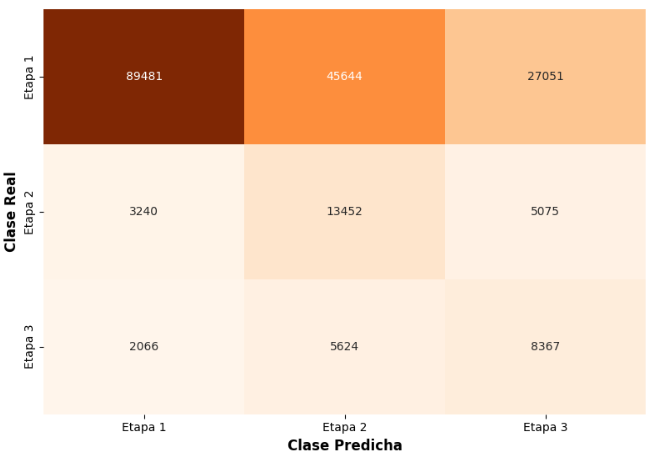
\includegraphics[scale=0.43]{imagenes/Capturas/graph-5-1.png}
	\caption{Matriz de Confusión Multiclase (Red Neuronal)}
	\vspace{-20pt}
\end{figure}

Como contraparte, la Precisión (\textit{Precision}) para las clases de riesgo se situó en un 21\%. Es decir, de cada cinco cohortes alertadas por el sistema, cuatro corresponden a un riesgo bajo. No obstante, desde la perspectiva de la gestión de riesgo, esto representa la estrategia de la que hablamos previamente: es preferible asumir los costos de pérdida de los Falsos Positivos, que absorber la pérdida total del capital por un incumplimiento no anticipado (Falsos Negativos).

\subsubsection{Curva ROC y Área Bajo la Curva (AUC)}
Para visualizar el desempeño discriminativo del modelo, se analizaron las curvas ROC bajo un esquema uno-contra-todos. La red neuronal alcanzó un AUC unificado y estable en el espectro de riesgo: 0.79 (Etapa 1), 0.76 (Etapa 2) y 0.78 (Etapa 3). 

\begin{figure}[H]
	\centering
	\vspace{0pt}
	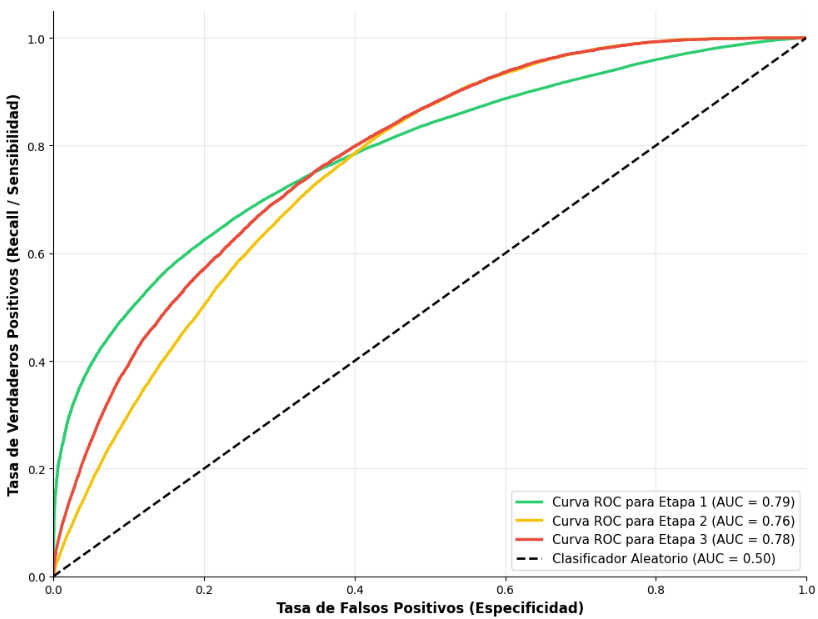
\includegraphics[scale=0.45]{imagenes/Capturas/graph-5-2.png}
	\caption{Curvas ROC Multiclase (One-vs-Rest)}
	\vspace{-10pt}
\end{figure}

Un AUC de 0.78 en la cartera deteriorada confirma que el modelo posee un 78\% de probabilidad de asignar un mayor puntaje de riesgo a una cohorte estadísticamente vulnerable frente a una cohorte estable. Lograr este grado de separación únicamente a través de demografía estática y características comerciales (sin consultar inflación o temporalidad) demuestra una alta eficacia de la arquitectura para la predicción de nuevas observaciones.



